% Define a new counter called thebox
\newcounter{box}
\newcounter{code}
% Define a custom environment for the mathematical model with a light violet background
\newenvironment{mathmodel}{
    \begin{tcolorbox}[colback=violet!5, colframe=white, sharp corners, boxrule=0pt, title=Mathematical Model of the Kinetic System]
}{
    \end{tcolorbox}
}

% Define a custom environment for the mathematical model with a light violet background
\newenvironment{mathmod}{
    \begin{tcolorbox}[colback=blue!5, colframe=white, sharp corners, boxrule=0pt, title=Mathematical Model of the Kinetic System]
}{
    \end{tcolorbox}
}

% Define a custom environment for code display
\newenvironment{codebox}{
    \begin{tcolorbox}[colback=gray!10, colframe=black, sharp corners, boxrule=0.5pt, title=Code Box]
}{
    \end{tcolorbox}
}

% Tables . use \table1{\textwidth}{caption 
% reference with \fullref{tab:table1}}
\def\ANOVA#1#2{
\begin{tableminipage}{#1}
\customlabel{tab:table1}{\textbf{Table 1}}~{#2}\\[1em]
\begin{tabularx}{\textwidth}{@{}lrrXXX@{}}
\hline
 & {\bf \centering \begin{minipage}[t]{3.5em}Sum of Sqares\end{minipage}} & {\bf df} & {\bf Mean Square} & {\bf F} & {\bf Sig.} \\
\hline
Between Groups & 37.609 & 3  & 12.536 & 45.385 & {\bf <.001}\\
Within Groups & 18.783 & 68 & 276 &  & \\
Total         & 56.392 & 71 &  &  & \\
\hline
\end{tabularx}
\end{tableminipage}
}

\def\WALLIS#1#2{
\begin{tableminipage}{#1}
\customlabel{tab:table2}{\textbf{Table 2}}~{#2}\\[1em]
\begin{tabularx}{\textwidth}{@{}XXrX@{}}
\hline
 {\bf \begin{minipage}{7.5em}Null Hypothesis\end{minipage}} & {\bf Test} & {\bf Sig.\footnote{The Significance level is .050}\footnote{Asymptotic significance is displayed}} & {\bf Decision}\\
\hline
 The distribution of the optical density at 595 nm is the same for INH, ETH, NCE and WT.& Independent-Samples Kruskal-Wallis Test & < .001 & Reject null hypothesis\\
\hline
\end{tabularx}
\end{tableminipage}
}


% Figures . use \figure1{0.35}{caption}
% reference with \fullref{fig:figure1}}
\def\imgtaskA#1{
\refstepcounter{figure} % Step the figure counter
\customlabel{fig:\thefigure}\\
\newline
%\begin{center}
    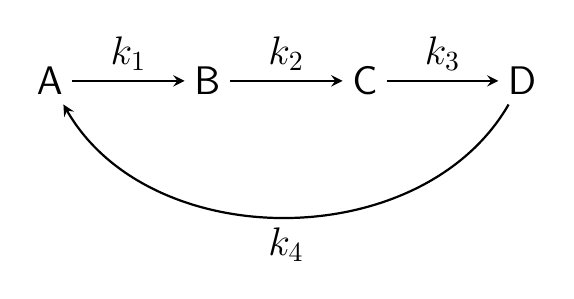
\begin{tikzpicture}[
      node distance=2cm,
      every node/.style={font=\sffamily\Large},
      arrow/.style={thick,->,>=stealth}
    ]
    
    % Nodes for substances
    \node (A) {A};
    \node (B) [right of=A] {B};
    \node (C) [right of=B] {C};
    \node (D) [right of=C] {D};
    
    % Arrows representing reactions
    \draw[arrow] (A) -- node[above] {$k_1$} (B);
    \draw[arrow] (B) -- node[above] {$k_2$} (C);
    \draw[arrow] (C) -- node[above] {$k_3$} (D);
    \draw[arrow] (D) to[bend left=60] node[below] {$k_4$} (A);
    
    \end{tikzpicture}
%\end{center}
\newline
\noindent\parbox[t]{0.48\textwidth}{\customlabel{fig:\thefigure}{\textbf{Figure \thefigure}} #1}\\[1em]
}

\def\circuit#1#2{
\refstepcounter{figure} % Step the figure counter
\begin{center}
\customlabel{fig:\thefigure}
\mbox{\includegraphics[scale = #1]{fig/s1b/imgtaskB.jpeg}}\\[0.3em]
\end{center}
\parbox[t]{\textwidth}{\customlabel{fig:figure2}{\textbf{Figure \thefigure.}} #2}\\[1em]
}
\def\imgtaskB_tikz#1{
\refstepcounter{figure} % Step the figure counter
\customlabel{fig:figure4}\\
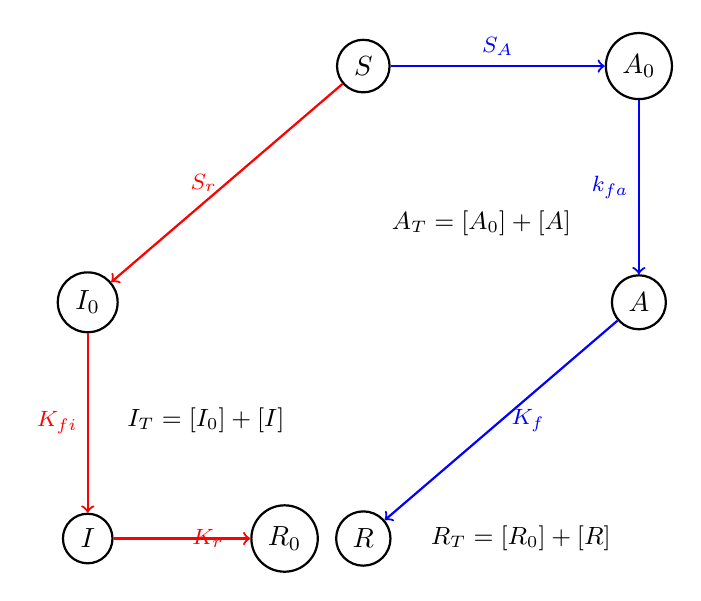
\begin{tikzpicture}
    % Nodes
    \node[circle, draw, thick] (S) at (0.5, 3) {$S$};
    \node[circle, draw, thick, fill=white] (I0) at (-3, 0) {$I_0$};
    \node[circle, draw, thick, fill=white] (I) at (-3, -3) {$I$};
    \node[circle, draw, thick, fill=white] (R0) at (-0.5, -3) {$R_0$};
    \node[circle, draw, thick, fill=white] (R) at (0.5, -3) {$R$};
    \node[circle, draw, thick, fill=white] (A0) at (4, 3) {$A_0$};
    \node[circle, draw, thick, fill=white] (A) at (4, 0) {$A$};

    % Reactions
    \draw[->, blue, thick] (S) -- node[midway, above] {\footnotesize $S_{A}$} (A0);
    \draw[->, red, thick] (S) -- node[midway, left] {\footnotesize $S_{r}$} (I0);
    \draw[->, red, thick] (I0) -- node[midway, left] {\footnotesize $K_{fi}$} (I);
    \draw[->, blue, thick] (A0) -- node[midway, left] {\footnotesize $k_{fa}$} (A);
    \draw[->, blue, thick] (A) -- node[midway, right] {\footnotesize $K_f$} (R);
    %\draw[<->, black, thick] (R0) -- node[midway, below] {\footnotesize $K_f$, $K_I$} (R);
    \draw[->, red, thick] (I) -- node[midway, right] {\footnotesize $K_r$} (R0);
    %\draw[->, blue, thick] (R) -- node[midway, below] {\footnotesize $k_{f}$} (R0);

    % Equations
    \node at (-1.5, -1.5) {\small $I_T = [I_0] + [I]$};
    \node at (2, 1) {\small $A_T = [A_0] + [A]$};
    \node at (2.5, -3) {\small $R_T = [R_0] + [R]$};
\end{tikzpicture}
\parbox[t]{0.48\textwidth}{\customlabel{fig:\thefigure}{\footnotesize\textbf{Figure \thefigure.}} #1}\\[1em]
}

\def\resultfig#1{
\refstepcounter{figure} % Step the figure counter
\customlabel{fig:\thefigure}\\
\begin{pspicture}(0,-5)(16,5)
    % Nodes for major steps
    \rput(2, 4){\rnode{ODESolver}{\psframebox[linewidth=1pt,fillstyle=solid,fillcolor=lightgray]{ODE Solver}}}
    \rput(2, 3.28){\rnode{ODESolverDetails}{\psframebox[linewidth=0.5pt,fillstyle=solid,fillcolor=white]{%
        \begin{tabular}{l}
            Numpy, SciPy (solve_ivp)\\ 
        \end{tabular}
    }}}
    
    \rput(7, 4){\rnode{DataGen}{\psframebox[linewidth=1pt,fillstyle=solid,fillcolor=lightgray]{Generated Data}}}
    \rput(7, 3.28){\rnode{DataGenDetails}{\psframebox[linewidth=0.5pt,fillstyle=solid,fillcolor=white]{%
        \begin{tabular}{l}
        Time-series generation (CSV) \\  
        \end{tabular}
    }}}
    
    \rput(7, 1){\rnode{MLTrain}{\psframebox[linewidth=1pt,fillstyle=solid,fillcolor=lightgray]{ML Model Training}}}
    \rput(7, 0.24){\rnode{MLTrainDetails}{\psframebox[linewidth=0.5pt,fillstyle=solid,fillcolor=white]{%
        \begin{tabular}{l}
        RandomForestRegressor\\ 
        \end{tabular}
    }}}
    
    \rput(12, 4){\rnode{Prediction}{\psframebox[linewidth=1pt,fillstyle=solid,fillcolor=lightgray]{Parameter Prediction}}}
    \rput(12, 3.28){\rnode{PredictionDetails}{\psframebox[linewidth=0.5pt,fillstyle=solid,fillcolor=white]{%
        \begin{tabular}{l}
        Predict \(k_1\)\cdots \(k_4\) \\ 
        \end{tabular}
    }}}
    
    \rput(12, 1){\rnode{SimODE}{\psframebox[linewidth=1pt,fillstyle=solid,fillcolor=lightgray]{Simulated ODE System}}}
    \rput(12, 0.24){\rnode{SimODEDetails}{\psframebox[linewidth=0.5pt,fillstyle=solid,fillcolor=white]{%
        \begin{tabular}{l}
        Matplotlib visualization
        \end{tabular}
    }}}
    
    % Connecting arrows for main flow
    \ncline[linewidth=2pt]{->}{ODESolver}{DataGen}
    \ncline[linewidth=2pt]{->}{DataGen}{MLTrain}
    \ncline[linewidth=2pt]{->}{MLTrain}{Prediction}
    \ncline[linewidth=2pt]{->}{Prediction}{SimODE}
    \ncline[linestyle=dashed,linewidth=1pt]{->}{SimODE}{MLTrain} % Feedback loop
    
    % Labels for main flow sections
    \uput[u](4.5,4.5){\textbf{Data Generation Step}}
    \uput[r](9,-1.6){\textbf{Feedback for Model Enhancement}}
    \uput[u](9.5,4.5){\textbf{Prediction and Optimization}}
    
    % Dotted lines for initial conditions and result visualization
    \psline[linewidth=0.5pt,linestyle=dotted]{<-}(2,2.75)(2,1)
    \uput[r](2,2){\small Initial Conditions}
    \psline[linewidth=0.5pt,linestyle=dotted]{->}(12,2)(14,2)
    \uput[r](14,2){\small Result Visualization}

    % Iterative feedback description
    \rput(7,-2.5){\rnode{FeedbackLoop}{\psframebox[fillstyle=solid,fillcolor=yellow]{Iterative Improvement}}}
    \rput(7,-3.3){\rnode{FeedbackDetails}{\psframebox[linewidth=0.5pt,fillstyle=solid,fillcolor=white]{%
        \begin{tabular}{l}
        \textbullet\ Model retraining  (scikit-learn) \\ 
        \end{tabular}
    }}}
    \ncline[linestyle=dashed,linewidth=1pt]{->}{SimODE}{FeedbackLoop}
    \ncline[linestyle=dashed,linewidth=1pt]{->}{FeedbackLoop}{MLTrain}
    
    % Add legend at the bottom of the figure with appropriate alignment
    \rput[bl](0, -5.0){%
        \psframe[fillstyle=solid, fillcolor=white](0,0.1)(14,0.8)
        \rput[bl](0.3, 0.3){\textbf{Legend}. Solid lines represent process flow, dashed lines represent feedback or iterative steps.}
    }
\end{pspicture}\\
\noindent\parbox[t]{\textwidth}{\customlabel{fig:\thefigure}{\footnotesize\textbf{Figure \thefigure.}} #1}\\[1em]
}
\def\mathmodelA#1{
\stepcounter{box} % Increase the counter
\customlabel{box:\thebox}\\
\begin{mathmodel}
    \textbf{Stochiometric Reaction Pathway (Task 1a):}
    \[
    A \xrightarrow{k_1} B \xrightarrow{k_2} C \xrightarrow{k_3} D \quad \text{with feedback} \quad D \xrightarrow{k_4} A
    \]

    \textbf{Reaction Kinetic Equations:}
    \begin{itemize}
        \item \textbf{Reaction 1:} \( A \xrightarrow{k_1} B \) (Second Order Kinetics)
        \begin{align*}
            \frac{d[A]}{dt} &= -k_1 [A][B] \quad \text{(Consumption of A, Catalysed by B)} \\
            \frac{d[B]}{dt} &= k_1 [A][B] \quad \text{(Creation of B, Catalysed by B)}
        \end{align*}

        %[Comment: Confirm if this autocatalytic behavior aligns with s1a-coursework or if a modification is needed.]%

        \item \textbf{Reaction 2:} \( B \xrightarrow{k_2} C \) 
        \begin{align*}
            \frac{d[B]}{dt} &= -k_2 [B] \quad \text{(Consumption of B to form C)} \\
            \frac{d[C]}{dt} &= k_2 [B] \quad \text{(Creation of C)}
        \end{align*}

        %[Comment: Check if the stoichiometric coefficient affects \( k_2 \) in your coursework model.]%

        \item \textbf{Reaction 3:} \( C \xrightarrow{k_3} D \) 
        \begin{align*}
            \frac{d[C]}{dt} &= -k_3 [C] \quad \text{(Consumption of C)} \\
            \frac{d[D]}{dt} &= k_3 [C] \quad \text{(Creation of D)}
        \end{align*}

        %[Comment: Ensure consistency in units and whether \( k_3 \) represents first-order kinetics.]%

        \item \textbf{Feedback Reaction:} \( D \xrightarrow{k_4} A \) 
        \begin{align*}
            \frac{d[D]}{dt} &= -k_4 [D] \quad \text{(Consumption of D)} \\
            \frac{d[A]}{dt} &= k_4 [D] \quad \text{(Recreation of A)}
        \end{align*}

        %[Comment: Clarify whether \( k_4 \) is dependent on any external control mechanisms.]%
    \end{itemize}

    \textbf{Complete ODE System:}
    \begin{align*}
        \frac{d[A]}{dt} &= -k_1 [A][B] + k_4 [D], \\
        \frac{d[B]}{dt} &= k_1 [A][B] - k_2 [B], \\
        \frac{d[C]}{dt} &= k_2 [B] - k_3 [C], \\
        \frac{d[D]}{dt} &= k_3 [C] - k_4 [D].
    \end{align*}

    \textbf{Explanation:}
    \begin{itemize}
        \item Mathematical model for the irreversable cyclic reaction pathway.
        \item Rate constants: (\( k_1, k_2, k_3, k_4 \)); Species: \(A,B,C,D\).
    \end{itemize}
\end{mathmodel}
\noindent\parbox[t]{\textwidth}{\customlabel{box:\thebox}{{\footnotesize\textbf{Box \thebox.}}} #1}\\[1em]
}

\def\steadystate#1{
\stepcounter{box} % Increase the counter
\customlabel{box:\thebox}\\
\begin{mathmodel}
\textbf{Equilibrium State:}
\begin{align*}
\text{Reaction: }  A \xrightarrow{k_1} B \xrightarrow{k_2} C \xrightarrow{k_3} D \\
\quad \text{Feedback:} \quad D \xrightarrow{k_4} A
\end{align*}

\textbf{ODEs for Steady State:}
\begin{align*}
    \frac{d[A]}{dt} &= -k_1 [A][B] + k_4 [D] = 0, \\
    \frac{d[B]}{dt} &= k_1 [A][B] - k_2 [B] = 0, \\
    \frac{d[C]}{dt} &= k_2 [B] - k_3 [C] = 0, \\
    \frac{d[D]}{dt} &= k_3 [C] - k_4 [D] = 0.
\end{align*}
\end{mathmodel}
\noindent\parbox[t]{\textwidth}{\customlabel{box:\thebox}{\footnotesize\textbf{Box \thebox.}} #1}\\[1em]
}
\def\steadystatedfc#1{
\stepcounter{box} % Increase the counter
\customlabel{box:\thebox}\\
\begin{mathmod}

\textbf{ODEs for Steady State:}
\begin{align*}
    \frac{d[A]}{dt} &= k_{fa} [S][A_0] - k_{-a} [A] = 0, \\
    \frac{d[I]}{dt} &= k_{fi} [S][I_0] - k_{-i} [I] = 0, \\
    \frac{d[R]}{dt} &= k_f [A][R_0] - k_r [I][R] = 0. \\
\end{align*}
\end{mathmod}
\noindent\parbox[t]{\textwidth}{\customlabel{box:\thebox}{\footnotesize\textbf{Box \thebox.}} #1}\\[1em]
}

\def\steadysolution#1{
\stepcounter{box} % Increase the counter
\customlabel{box:\thebox}\\
\begin{mathmodel}
\textbf{Steady-State 1:}
\begin{align*}
    A = \text{const.}, & B = C = D = 0
\end{align*}
\textbf{Steady-State 2:}
\begin{align*}
    A = \frac{k_2}{k_1}, & B = [D] \frac{k_4}{k_2}, & C = [D] \frac{k_4}{k_3}, & D = \text{const.}.
\end{align*}

\end{mathmodel}
\noindent\parbox[t]{0.48\textwidth}{\customlabel{box:\thebox}{\footnotesize\textbf{Box \thebox.}} #1}\\[1em]
}

\def\steadysolutiondfc#1{
\stepcounter{box} % Increase the counter
\customlabel{box:\thebox}\\
\begin{mathmod}
    \textbf{Steady-States:}
    \begin{align*}
        \text{Steady State for } A: & \quad A = \frac{A_0 S k_{fa}}{k_{-a}}, \\
        \text{Steady State for } I: & \quad I = \frac{I_0 S k_{fi}}{k_{-i}}, \\
        \text{Steady State for } R: & \quad R = \frac{A_0 R_0 k_{-i} k_{f} k_{fa}}{I_0 k_{-a} k_{fi} k_{r}}.
    \end{align*}
\end{mathmod}
\noindent\parbox[t]{0.48\textwidth}{\customlabel{box:\thebox}{\footnotesize\textbf{Box \thebox.}} #1}
}

\def\steadysolutionrs#1{
\stepcounter{box} % Increase the counter
\customlabel{box:\thebox}\\
\begin{mathmod}
    \textbf{Steady-States R(S)}
    \setcounter{equation}{0} % Reset the equation counter
    \begin{align}
        &R(S) = \frac{A R_0}{I} \cdot \frac{k_{f}}{k_{r}}, \\[5pt]
        &R_{\text{forward}}(S) = \frac{A R_0 S}{I} \cdot \frac{k_{f}}{k_{r}}, \\[5pt]
        &R_{\text{reverse}}(S) = \frac{A R_0 S}{I} \cdot \frac{k_{f} k_{fa}}{k_{r} k_{-a} k_{fi}}.
      \end{align}
\end{mathmod}
\noindent\parbox[t]{0.48\textwidth}{\customlabel{box:\thebox}{\footnotesize\textbf{Box \thebox.}} #1}
}

\def\reactionprocess#1{
\stepcounter{box} % Increase the counter
\customlabel{box:\thebox}\\
\begin{mathmod}
\textbf{Stoichiometric Reactions (\fullref{fig:2})}\\[2em]
\textbf{Reaction 1. Enzyme \( A \) - Kinetics:}
\begin{align*}
    \text{Feedforward Reaction:} & \quad S + A_0 \xrightarrow{k_{fa}} S + A \\
    \text{Reverse Reaction:} & \quad A \xrightarrow{k_{-a}} A_0
\end{align*}

\textbf{Reaction 2. Enzyme \( I \) - Kinetics:}
\begin{align*}
    \text{Feedforward Reaction:} & \quad S + I_0 \xrightarrow{k_{fi}} S + I \\
    \text{Reverse Reaction:} & \quad I \xrightarrow{k_{-i}} I_0
\end{align*}

\textbf{Reaction 3. Conversion of \( R_0 \) to \( R \) Catalyzed by \( A \) and \( I \):}
\begin{align*}
    \text{Activation by \( A \):} & \quad R_0 \xrightarrow{k_{f}} R \\
    \text{Deactivation by \( I \):} & \quad R \xrightarrow{k_{r}} R_0
\end{align*}

\textbf{Total Enzymes:}
\begin{align*}
    A_T &= [A_0] + [A] \\
    I_T &= [I_0] + [I] \\
    R_T &= [R_0] + [R]
\end{align*}
\end{mathmod}
\noindent\parbox[t]{\textwidth}{\customlabel{box:\thebox}{\footnotesize\textbf{Box \thebox.}} #1}\\[1em]
}

\def\dualfeedforward#1{
\stepcounter{box} % Increase the counter
\customlabel{box:\thebox}\\
\begin{mathmod}
\textbf{Mathematical Modelling: Dual Feedforward Cuircuit (\fullref{fig:3})}
\[
S \rightarrow A_0 \xrightarrow{k_{fa}} A \xrightleftharpoons[k_{-a}]{} A_0, \quad S \rightarrow I_0 \xrightarrow{k_{fi}} I \xrightleftharpoons[k_{-i}]{} I_0, \quad A + R_0 \xrightarrow{k_f} R, \quad I + R \xrightarrow{k_r} R_0
\]

\textbf{Reaction Kinetic Equations:}
\begin{itemize}
    \item \textbf{Activation of \( A \)}:
    \[
    \frac{d[A]}{dt} = k_{fa} [S][A_0] - k_{-a} [A] \quad (\text{Activation of \( A_0 \), Deactivation of \( A \)})
    \]

    \item \textbf{Activation of \( I \)}:
    \[
    \frac{d[I]}{dt} = k_{fi} [S][I_0] - k_{-i} [I] \quad (\text{Activation of \( I_0 \), Deactivation of \( I \)})
    \]

    \item \textbf{Conversion of \( R_0 \) to \( R \) (Catalyzed by \( A \))}:
    \[
    \frac{d[R]}{dt} = k_f [A][R_0] - k_r [I][R] \quad (\text{Production of \( R \), Consumption of \( R \)})
    \]
\end{itemize}

\textbf{Complete ODE System:}
\[
\begin{aligned}
\frac{d[A]}{dt} &= k_{fa} [S][A_0] - k_{-a} [A], \\
\frac{d[I]}{dt} &= k_{fi} [S][I_0] - k_{-i} [I], \\
\frac{d[R]}{dt} &= k_f [A][R_0] - k_r [I][R].
\end{aligned}
\]

\textbf{Explanation:}
\begin{itemize}
    \item Reaction dynamics (Activation vs. Deactivation) of Enzyme species \( A, A_0, I, I_0, R \text{and} R_0 \).
    \item Rate constants: \( k_{fa}, k_{-a}, k_{fi}, k_{-i}, k_f, k_r \)
\end{itemize}
\end{mathmod}
\noindent\parbox[t]{\textwidth}{\customlabel{box:\thebox}{\footnotesize\textbf{Box \thebox.}} #1}\\[1em]
}


\endinput